\documentclass[11pt]{article}
\usepackage{geometry}                
\geometry{letterpaper}                   

\usepackage{graphicx}
\usepackage{hyperref}
\usepackage{amssymb}
\usepackage{epstopdf}
\usepackage{natbib}
\usepackage{amssymb, amsmath}
\DeclareGraphicsRule{.tif}{png}{.png}{`convert #1 `dirname #1`/`basename #1 .tif`.png}

%\title{Interdependent Evolution of Non-Spectral Opinions and Social Networks}
%\author{Fabian Rußmann, Stefan Rustler}
%\date{date} 

\usepackage{algorithm2e}
\usepackage{float}

\usepackage{color}
\definecolor{dkgreen}{rgb}{0,0.6,0.1}
\definecolor{gray}{rgb}{0.5,0.5,0.5}
\definecolor{mauve}{rgb}{0.58,0,0.82}
\definecolor{red}{rgb}{1,0,0}
\definecolor{blue}{rgb}{0,0,1}

\usepackage{listings}
\lstset{language=Matlab}
\lstset{breaklines=True}
\lstset{basicstyle=\footnotesize, numbers=left, numberstyle=\tiny, stepnumber=1}
\lstset{keywordstyle=\color{blue}, commentstyle=\color{dkgreen}, stringstyle=\color{mauve}, numberstyle=\color{gray}}



\bibpunct{[}{]}{;}{a}{,}{,}

\begin{document}



\thispagestyle{empty}

\begin{center}
\includegraphics[width=5cm]{ETHlogo.eps}

\bigskip


\bigskip


\bigskip


\LARGE{ 	Lecture with Computer Exercises:\\ }
\LARGE{ Modelling and Simulating Social Systems with MATLAB\\}

\bigskip

\bigskip

\small{Project Report}\\

\bigskip

\bigskip

\bigskip

\bigskip


\begin{tabular}{|c|}
\hline
\\
\textbf{\LARGE{Opinion Formation: Impacts of convincing}}\\
\textbf{\LARGE{extreme individuals onto a society that typically}}\\
\textbf{\LARGE{converges to one opinion}}\\
\\
\hline
\end{tabular}
\bigskip

\bigskip

\bigskip

\LARGE{Alexander Stein, Niklas Tidbury \& Elisa Wall}



\bigskip

\bigskip

\bigskip

\bigskip

\bigskip

\bigskip

\bigskip

\bigskip

Zurich\\
December 2017\\

\end{center}



\newpage

%%%%%%%%%%%%%%%%%%%%%%%%%%%%%%%%%%%%%%%%%%%%%%%%%

\newpage
\section*{Agreement for free-download}
\bigskip


\bigskip


\large We hereby agree to make our source code for this project freely available for download from the web pages of the SOMS chair. Furthermore, we assure that all source code is written by ourselves and is not violating any copyright restrictions.

\begin{center}

\bigskip


\bigskip


\begin{tabular}{@{}p{3.3cm}@{}p{6cm}@{}@{}p{6cm}@{}}
\begin{minipage}{3cm}

\end{minipage}
&
\begin{minipage}{6cm}
\vspace{2mm} \large Fabian Russmann

 \vspace{\baselineskip}

\end{minipage}
&
\begin{minipage}{6cm}

\large Stefan Rustler

\end{minipage}
\end{tabular}


\end{center}
\newpage

%%%%%%%%%%%%%%%%%%%%%%%%%%%%%%%%%%%%%%%



% IMPORTANT
% you MUST include the ETH declaration of originality here; it is available for download on the course website or at http://www.ethz.ch/faculty/exams/plagiarism/index_EN; it can be printed as pdf and should be filled out in handwriting


%%%%%%%%%% Table of content %%%%%%%%%%%%%%%%%

\tableofcontents

\newpage

%%%%%%%%%%%%%%%%%%%%%%%%%%%%%%%%%%%%%%%



\section{Abstract}


The question whether our social network shapes the opinion we hold or whether our opinions determine who is part of our network, was central to this work. A model that simulates the interdependent evolution of non-spectral opinions and social networks was implemented by including both mechanisms of one's social network shaping one's opinion and vice-versa. We were able to show that by merely altering the reconnection probability $\Phi$ that determines which of the two mechanisms is favored, a phase transition of the opinion distribution can be observed at the critical point of $\Phi_c=0.32 \pm 0.05$. In one phase a giant cluster of equal opinion forms, whereas in the other there are only several smaller clusters. Attempts were made to describe this critical behavior in terms of solid state physics. We could show that different network sizes have the same critical point. Further a response function, the average time to reach consensus in the network, that diverges at the critical point could be identified. Finally, results were compared to hand-picked empirical data to give an idea of the applicability of our results.


\section{Introduction}

In this work, we investigated the dynamics of opinion and network formation. Both of these topics have received significant attention in the social sciences. Recently, however, other disciplines have also dealt with such problems, often applying models and methods of analysis from the physical sciences to social problems. Such studies have made quite some advances in the study of complex networks, (a good summary being given by \cite{review}), but have also dealt with the problem of network dynamics and opinion formation, for example in voter models \cite{voter model small world, voter model 2} \\


The process of opinion formation is arguably one of the most complex but also one of the most fundamental in sociology, with wide-ranging implications in politics, economics and social psychology. For example, questions such as "How do the landscape of political parties and election results evolve?", "Why and how did different religions emerge in the course of history?", "How do traders decide which stocks to buy or sell?" or "Why do people prefer to buy certain brands over others?" could all be described as problems of understanding opinion formation. Though these are admittedly very difficult challenges, an understanding of these questions could potentially allow us to influence (for the better or worse) the processes of opinion and belief formation. \\


In this work, we want to study an opinion and network formation process using a quantitative model. Of course, as any model, it will only provide a stark simplification and idealization of the problem. However, in contrast to a lot of existing studies on opinion formation and the dynamics of social networks, this work is unique in the sense that it proposes a model combining these two approaches: We want to study the mechanisms of people forming opinions while connected with other people. Hence we not only study how opinions evolve in a social setting, but we also allow the network itself to be adaptable to the opinions existing on it, making two interdependent forces of network evolution and opinion formation measurable. In a sense, we want to address the question: \\


\textbf{Does our social network shape the opinion we hold or does our opinion determine who is part of our network?} \\


The motivation for this project involves two different angles on very fundamental dynamics of our society. First of all, the social sciences try to understand the ways in which humans become who they are under the influence of their environment. How do people form their opinions, values, and beliefs and how do their friends and acquaintances play a role in this? Secondly, we are interested in the way our networks of friends and social ties form in the first place. How and why do we choose to be friends with certain people and not with others? How do networks of people in a society form?
From an intuitive point of view (considering that we are all social beings) most people would argue that the two aspects are interdependent or even that they are two extremes of the same process: Our social environment certainly shapes what we believe and which opinions we hold, while in turn our own values and opinions influence whom we choose to connect with and make part of our social network. On the basis of this rather vague but plausible assumption, our project is an attempt to disentangle and study the effects of these two mechanisms by the means simulations on networks with opinion attributes. \\


An example of a system that one would expect to be subject to such behavior is religious affiliation within a society. It could be argued that the social surroundings have an effect on (or, as an extreme, completely determine) which religion a person chooses to belong to. However, one's religion also influences to whom we connect with socially, for example through the community in a church (the opposing extreme would be that a person's social ties are entirely composed of members of the same religion). 

A different example, as mentioned above, is brand loyalty. Especially in cases where the quality of different products on the market is arguably very similar, social processes strongly influence one's decision in favor of a certain brand. Recent examples of this are smartphone brands, operating systems or browsers for computers but also more traditional examples such as car brands. Interestingly, brand loyalty in these cases has often been compared to religious mindsets. \\


In this context, it is also evident that the notion of "opinion" in this work is seen as a more generalized one: An opinion could be a religious belief, affiliation to a political party, preference for a certain brand etc. Also the definition of nodes and edges in a graph can be seen as much more general than just an individual in a network of personal acquaintances. In the example of religion for example, a node could be a family and "adapting an opinion" could mean a member of the family marrying someone of different religion, thereby changing the family's religious affiliation on the time scale of generations.

Another concrete restriction due to the definition of our model (see section \ref{sec:initial}) is that it only describes mutually exclusive, "non-spectral" opinions, i.e. an individual can hold one and only one opinion which is independent of all other opinions (i.e. there are no similar opinions). The above examples can be seen as roughly falling into these categories. An interpretation in terms of political views is difficult, however, since political opinions are multi-dimensional (a person can have several opinions on different aspects of political life) and of spectral nature (some views or parties are similar to each other). \\


\section{The Model}
\label{Sec:Model}

\subsection{Initial Setup}
\label{sec:initial}

In this work the network of opinion holders will be modeled by means of a graph with $N$ nodes and $M$ edges connecting the nodes. Thus "graph" in this context is a collection of edges and nodes and not to be confused with graphs of functions. The entire model is based on the work of P. Holme and M. E. J. Newman \cite{main paper}.\\


Each node represents an opinion holder, e.g. a single person, indexed by $i$, to whom a certain opinion $g_i$ is randomly assigned. The number of all possible opinions $G$ is only limited by the number of nodes $N$ existing in the network to a certain factor $\gamma = \frac{N}{G}$, where $\gamma > 1$. In this sense, it is not possible for every single individual to hold a unique opinion. In this model we are externally setting $\gamma$, i.e. the initial average number of nodes with the same opinion, as opposed to the number of existing opinions.\\ 

										
It is important to point out the nature of opinions this model assumes. Though different opinions will be denoted by a set of subsequent integers given by $G$, this is not to be mistaken with a spectrum of opinions with two extremes. That is no opinion is more similar to another than yet another. Each opinion is equally likely to be adopted by an opinion holder. This will have important implications on the type of empirical data the results of this model can be compared to, as already alluded to in the introduction.\\


The edges that connect two nodes represent a bridge of interaction of two nodes, i.e. direct interaction can only occur between two connected nodes. In general an individual edge can be directed, which means that information can only be carried from one node to another along its direction. In our model each connection will be undirected, i.e. two nodes can influence \textit{each other}. In contrast to \cite{main paper}, we have forbidden self-edges and multi-edges to occur, as this is typical for acquaintance networks. In this sense a node as such is already connected to itself and can also not connect with certain nodes more strongly than with others via more edges. The number of edges leaving a node $i$ is given by the degree $k_i$. The average degree of the graph is therefore given by $k_{avg}=\frac{2M}{N}$. By externally setting $N$ and $k_{avg}$, edges are distributed in a random and uniform fashion: each pair of nodes is equally likely to be connected by an edge. This random graph generation was first proposed by Paul Erdos and Alfred Renyi \cite{erdos renyi}. There are many other types of graphs but due its simplicity and wide applicability, this work focusses on random graphs of different sizes.\\


Even though we are using the interpretation of nodes and edges as people with opinions and social connections for reasons of intuition, it is important to not restrict the notion of connected and interacting nodes to such a specific context. The concept of nodes holding and influencing each other's opinion is much broader as mentioned in the introduction.\\

\subsection{Time Evolution Algorithm}
\label{Sec:TimeEvol}

The above-mentioned setup of nodes, edges and opinions is now subject to time-evolution. Specifically, nodes are allowed to interact such that a \textit{co}evolution of edges and opinions occurs: 

In two basic update steps, we will enable each node to follow one of the two mechanisms, reconnecting to a node of equal opinion \textit{or} adapting his/her opinion to the neighborhood. A tunable probability $\Phi$ of choosing either one of them will be included in the model. In this work this probability will be referred to as \textit{reconnection probability}. In more detail, at each time step the following will be done:

\begin{enumerate}
\item Pick a random node $i$ with opinion $g_i$. 
\item If $k_i=0$, start over at step 1. 
\item With probability $\Phi$ select at random one of the nodes $j$ that $i$ is connected to.

a. If $g_i = g_j$, start over at step 1.

b. Otherwise, reconnect to a randomly chosen $j'$ of same opinion, i.e. $g_{j'} = g_i$.

\item Otherwise, with probability $1-\Phi$ randomly select one of the neighboring vertices $j$ and change $g_i$ to $g_j$.
\end{enumerate}

Here the third step corresponds to the mechanism in the network of an individual reconnecting to like-minded individuals, whereas the fourth step to that of an individual adapting his/her opinion to his/her neighborhood. 

Steps 1. to 4. are iteratively performed until a convergent or equilibrium state is achieved. The attentive reader might have noticed in the steps above that step 3a could result in an infinite loop as soon as every node is only connected to nodes of equal opinion. This is exactly the definition of the convergent state and will be referred to as the \textit{consensus state}. We will be mainly concerned with how this convergent state looks like. Separated clusters of different opinions will have formed, whose size distribution in dependence of several external parameters, namely $\Phi$, $N$ and $k$, this work is mainly concerned with.\\


Intuitively, one can picture two extreme scenarios: one in which there is one prominent opinion, and one in which there is no such opinion but several much less prominent ones. In other words, an emergent phenomenon of different manifestation is to be expected as macroscopic outcome from the microscopic steps described above.


\section{Theory of Critical Phenomena}
\label{Sec:Theory}

Several analogies can be drawn from the system of interacting nodes to systems in solid state physics. Therefore some formulas and concepts of this field will be applied in this work, all of which will be derived in this section and translated to our case. The works of \cite{ASSP} and \cite{Nolting} served as main source for this. The derivations in this section are also motivated by an attempt to understand the formulas stated in \cite{main paper} without further derivation. It has to be stressed that some analogies arise from assumptions made that would in fact need further justifications and investigations which go beyond the scope of this work.\\


As indicated in the previous section, two extreme scenarios are possible in the opinion network. Speaking in physics terms, two phases that can transition into each other are expected to occur. An individual phase is characterized by several internal parameters, most importantly the so-called \textit{order parameter}. In this sense one can also speak of an \textit{ordered} and \textit{unordered} state. If at some point this parameter changes drastically upon slight variation of another external parameter, one can speak of a \textit{phase transition}. This point of drastic change is called the \textit{critical point}. This sensitive response or criticality of the system typically manifests itself in a divergence of response function. One can also speak of a divergence of the \textit{coherence length}, meaning that the effect of a slight change at some point in the system can influence the whole system. 

A simple example is the boiling of water. Upon slight variation of the (external) temperature near the boiling point, a drastic change of (internal) density is observed: the unordered liquid state transitions into an ordered gaseous state. In this work the external variable will be the reconnection probability $\Phi$, whereas the internal order parameter will be the relative size of the biggest opinion cluster, denoted by $S$. The critical point at which the phase transition occurs will be denoted by $\Phi_c$. Further, the two phases occuring will be referred to as the \textit{unordered} and \textit{ordered phase}, the latter of which being marked by a high value of the order parameter $S$.\\


The behavior of a system near its critical point is characterized by a single quantity, the dimensionless \textit{critical exponent}. These exponents are at the heart of the theory of critical phenomena. According to this theory, any physical quantity that is dependent on a specific external parameter follows a power law close to the critical value of this external parameter. In statistical physics, for example, all quantities that depend on temperature would behave the same way close to the critical temperature. Therefore, there is exactly one critical exponent per external parameter. How close the system is to the critical point is generally expressed by a \textit{reduced} quantity, e.g. the reduced temperature $\tau = \frac{T-T_c}{T_c}$. In our case we will define the reduced reconnection probability likewise as

\begin{equation}
\varphi = \frac{\Phi - \Phi_c}{\Phi_c}.
\end{equation}

The dependent variable is the relative maximal cluster size $S(\varphi)$. Its behavior near the critical point $\Phi_c$ is described by

\begin{equation} \label{Eq:powlaw}
S(\varphi) \sim |\varphi|^\alpha.
\end{equation}

The tilde is read as "behaves as" for $\varphi \rightarrow 0$. The absolute value is based on the general observation that the direction from which the critical point is approached, does not matter. In this work we do not test this equivalence. The critical exponent is denoted by $\alpha$. It turns out that seemingly very different systems have the same critical exponent and therefore behave the same way near the critical point. According to the hypothesis of universality, they are said to belong to the same universality class uniquely defined by one critical exponent for each external parameter. In our case we do only vary one external parameter, i.e. the reconnection probability, for which we can determine the critical exponent and check which universality class it belongs to. The universal critical exponent itself is only dependent on the following:

\begin{enumerate}
\item Dimensionality $d$ of the system
\item Range of interaction
\item Spin dimensionality (irrelevant in our case)
\end{enumerate}

Translating all of these dependencies to our case is rather difficult. The dimensionality of a graph that carries no spatial information and in which each site can interact with every other site, unlike a regular crystal lattice for example, cannot be pictured easily if at all. The case is simpler with the range of interaction. The concepts presented in this section are based on an ideal system of infinite size (thermodynamic limit). If we limit the size of our system, i.e. we set $N$ to a certain finite value, the range of interaction that would usually diverge (response functions diverge) at the critical point is limited by $N$. It is therefore to be expected that for different network sizes different critical exponents will be obtained. This will manifest in lines of different slopes intersecting in the critical point in a log-log plot.

This issue solved with the so-called scaling law that enables us to correct for different system sizes and extract one single critical exponent $\alpha$ according to \eqref{Eq:powlaw} that is independent of the size of the system. In the following we will derive this relation and state how the critical exponent can be determined.\\


In the context of statistical physics all functions of quantities that undergo a phase transition, are some derivative of the free energy $F$ of the system that has to be minimized in order form a low energy ground state, i.e. a new phase. In our case the ground state is the consensus state, which is of low energy in a sense that no disagreeing nodes are connected. We further assume that the maximal cluster size is some derivative of $F$. It can be proven that the free energy must be a generalized homogeneous function that follows

\begin{equation}
F(\lambda^x \varphi) = \lambda F(\varphi),
\end{equation}

where $\lambda$ is some real scalar that we can set to $N^d$, where $d$ is the dimensionality of the system. Here $x$ denotes some exponent of which the critical exponent will be dependent. Further we need to consider the free energy \textit{density} that is independent of the system size. We get

\begin{equation}
f(N^x \varphi) = N^d f(\varphi),
\end{equation}

which can be derived with respect to its only internal parameter $\varphi$ to get

\begin{equation}
N^{x-d} \cdot \frac{\partial f(N^x \varphi)}{\partial N^x \varphi} = \frac{\partial f(\varphi)}{\partial \varphi}.
\end{equation}

In the next step we are assuming that $\frac{\partial f(\varphi)}{\partial \varphi} = S(\varphi)$. This step is by no means trivial and needs further justification. However, it leads to equation (1) in the work of \cite{main paper} that was used for determining the critical exponent and will be employed in this work as well. We can thus write

\begin{equation}
S(\varphi) = N^{x-d} S(N^x\varphi)
\end{equation}

or to make it more comparable to \cite{main paper},

\begin{equation}\label{Eq:1paper}
N^{a} S(\varphi) = S(N^b\varphi).
\end{equation}

This equation will be used to extract the values of $a$ and $b$ from curves of $S(\varphi)$ of different $N$. In order to get the critical exponent, \eqref{Eq:1paper} has to be put into the form of \eqref{Eq:powlaw}. In order to do so, it can be chosen that $N = \varphi^{-1/b}$ such that $S(1)=const.$ The power law behaviour of $S(\varphi)$ is therefore given as

\begin{equation}
\label{Eq:ab-powlaw}
S(\varphi) \sim |\varphi|^{\frac{a}{b}} =: |\varphi|^\alpha.
\end{equation}



\section{Implementation}

The model described in section \ref{Sec:Model} was implemented and simulated with MATLAB\textsuperscript{\textregistered} (Version R2012b). This section will outline the structure of our implementation and data organization by using pseudocode. \\


At the heart of our implementation lies the representation of a network of $N$ nodes and an opinion distribution using matrices and vectors, respectively. An $N$x$N$ matrix $A_{ij}$ with entries 1 or 0 was used to represent existing or non-existing connections between nodes $i$ and $j$. The entries could take binary values only as multi-edges were not considered. Since only undirected nodes were allowed, the matrix was perfectly symmetric, i.e. a connection between $i$ and $j$ was written as both the $(i,j)$ and the $(j,i)$ entry being equal to 1. Self-edges were also disallowed, so the matrix diagonal was 0 by definition. Hence, all valuable information is carried in the upper triangle of the matrix. 

Different opinions were simply labeled as subsequent integers into a vector of length $N$ with the indices of the vector representing the nodes.

\subsection{Main Script}

Upon implementing the model, a functional programming approach was taken in which logically closed subroutines (e.g. the generation of a random network or the time evolution steps of a graph) were written as closed, independently callable functions. All functions and commands necessary to carry out the simulation were called from a "main script" file, which was the script executed to start the simulation. The structure of this main script is outlined in Algorithm \ref{main_script pseudo}.\\


\begin{algorithm}[H]
\label{main_script pseudo}
 \SetAlgoLined
 \KwIn{$k_{avg}$,  \gamma, N_{range}, $\Phi_{range}$, $runs$}
 \ForEach{N in N_{range} }
	{
	generate random graph\;
	generate random opinion distribution\;
	both are kept constant for one N\;
	\ForEach{$\Phi$ in $\Phi_{range}$ }
		{
		\ForEach{run in runs }
			{
			execute simulation\;
			sum up results\;
			}
		average over results\;
		save results\;	
	
	
		}
		
	}	


 \caption{Structure of main script}
\end{algorithm}

\parskip 11pt

First the input parameters, which are the average degree $k_{avg}$, the average number of nodes per opinion $\gamma$, and parameter ranges for different system sizes $N$ and $\Phi$ that are defined in the beginning. Then the different system sizes are looped over whereas one random graph and one random opinion distribution are generated for each system size and kept for that iteration to ensure consistency. With this initial network, the range of $\Phi$ is iterated over. For each $\Phi$, the time evolution is executed a specified number of times in order to be able to calculate average values of the results. The results, above all the cluster size distribution and the order parameter, are then saved. Saving usually included only the average values since saving for each individual run would have created unnecessary large amounts of data, although this is useful in the beginning to ensure the simulation is operating correctly.


\subsection{Random Graph Generation}

Generating a random graph is a seemingly simple task, even with the restrictions of our model (no self- and multi-edges allowed) being taken into account. Since we needed the number of edges in the network to be exactly as specified, the \textit{uniform} $G(N,M)$-variant was chosen over the $G(N,p)$-variant of Erd\H{o}s-R\'{e}nyi algorithm \cite{erdos renyi}. In the latter variant $k_{avg}$ would be subject to small fluctuations. As we were going to investigate critical phenomena that are potentially very sensitive to changed in the external parameters, we wanted to make sure to exclude such fluctuations and wrote our own uniform random graph generator as shown in algorithm \ref{graph_gen pseudo}.\\

\begin{algorithm}[H]
\label{graph_gen pseudo}
 \SetAlgoLined
 FUNCTION\;
 \KwIn{$N$, $M$}
 \KwOut{$A_{ij}$}
 initialize empty matrix\;
 initialize $counter$\;
\While{counter \leq M}
	{
		choose random i\;
		choose random j\;
		
		\If{($i$ == $j$)  or  ($i,j$ already connected)}
		{
			continue\;
		}
		\Else
		{
			set $A_{ij}$ and $A_{ji}$ to 1\;
			increment $counter$\;
		}
	}


 \caption{Generation of a random graph}
\end{algorithm} \\


The pseudocode is fairly simple and straightforward. A randomly chosen pair $i,j$ is connected symmetrically (in both directions) unless $i = j$ (self-edges forbidden) or $i$ and $j$ are already connected. Using a counter and a while-loop, we made sure that exactly $M$ edges are placed randomly.

The generation of an initial opinion vector is in fact very simple. For each entry of the opinion vector, one of $G$ possible opinions is selected at random.

\subsection{Simulation Script}

The central feature of our model is the time evolution of the network and its opinion structure. Though the steps of updating the network have already been described in section \ref{Sec:TimeEvol}, some of the exact details of the process are actually not trivial to implement in Matlab. Thus, for reasons of reproducibility, the time evolution of the simulation is presented here in pseudocode \ref{simulation pseudo} and the important details are clarified in words.

The outermost loop represents the iteration over time steps. This needs to be a while loop since we want to keep updating until a consensus state has been reached, which occurs after some previously unknown convergence time $t$.

It is important to note that at each time step, we \emph{first} perform a check as to whether or not the consensus state has already been reached. This is because we continue the loop (i.e. pick a new $(i,j)$ pair) each time $i$ and $j$ by chance already have the same opinion. If we were to check for the convergence after choosing $i$ and $j$, we would eventually get stuck in an infinite loop. The decision of not letting $i$ and $j$ interact if they are already of the same opinion is by no means a trivial one and stands in contrast to \cite{main paper}, as discussed in section \ref{Sec:TimeEvol}.

On the basis of performance optimization, the check for a consensus state is formulated in a negative way, i.e. we break the convergence check if any pair of connected nodes is \emph{not} of the same opinion: We do not need to waste time and iterate through all other pairs of neighbors if even a single one is not of the same opinion. One such pair is enough to conclude that no consensus has been reached yet.

Another non-trivial technicality is to require a pair of potential new connection $(i,j')$ to not be already connected. Otherwise, i.e. if they are already connected, we would overwrite this existing connection whilst deleting the old one. This would decrease the total number of edges $M$ in the network, which needs to be constant.


\begin{algorithm}[H]
\label{simulation pseudo}
 \SetAlgoLined
 FUNCTION\;
 \KwIn{$A_{ij}$, opinion vector, $N$, $\Phi$}
 \KwOut{$A_{ij}$, opinion vector, convergence time $t$}
 initialize convergent state binary $abort$ ; initialize $t$\;
\While{convergent state not reached}
	{
		\tcc*[h]{Check if convergent state has been reached:}\;
		
		\ForEach{node $x$ in $N$}
			{
				\ForEach{node $y$ connected to $x$}
					{
						\If{opinion($x$) != opinion($y$)}
							{
								no convergent state reached\;
								break out of convergence check loops, continue at time evolution\;
							}
						\Else
							{
								set $abort$ binary to indicate that convergence has been reached\;
							}
					}
			}
		
		\tcc*[h]{Perform time evolution:}\;
		increment $t$\;
		pick random node $i$\;
		\If{$i$ is at all connected to any other node}
			{
				pick random node $j$ that is connected to $i$\;
				\If{opinion(i) == opinion(j)}
					{
						continue, i.e. pick new $i,j$ pair and start over\;
					}
				\If{probability $\Phi$}
					{
						pick random node $j'$ out of nodes with same opinion as $i$\;
						\If{$i$ and $j'$ NOT already connected}
							{
							delete connection between $(i,j)$\;
							establish new connection between $(i,j')$\;
							}
					}
							
				\Else(probability $1-\Phi$)
					{
					Set opinion($i$) = opinion($j$)\;
					}
					
					
					
			}
	}
	


 \caption{Simulation Function: Time Evolution of Network and Opinion Structure}
\end{algorithm} \\



\subsection{Optimization and Data Storage}

Several means of increasing computation and storing efficiency have been realized. Pre-defined MATLAB functions have been employed wherever possible. To save memory, sparse adjacency matrices have been used instead of full ones. As already mentioned in the previous subsection, we optimized our simulation function such that unnecessary iterations are broken off early, e.g. when checking for a convergent state or upon having chosen two nodes of already equal opinion. \\

Our main script is in principle parallelizable as the two input parameters that we varied ($N$ and $\Phi$) are producing independent data points in the parameter space. Though we did not use the parallelization toolbox, we usually ran multiple MATLAB sessions at the same time to take advantage of multi-core processors. We also prepared a version of our simulation that is executable on ETH's Brutus cluster (see appendix), but were not able to take full advantage of it due to missing licenses of the frequently used bioinformatics toolbox. \\

As already mentioned above, functions have been logically separated into initial generation, time evolution, and data saving. Plotting and analysis were performed after the simulations had finished. For this, the entire workspace after the simulation was saved to a file. The file was named with a string containing the parameter combinations that were used in order to keep an overview. This string was also used by the different plotter scripts to open and analyze data for a desired combination of input variables. When creating some plots, e.g. the (rescaled) order parameter vs. $\varphi$ or the average convergence time, the entire data was loaded and plotted by "walking through" the data output directory. Though this process could have been improved, we did not spend too much time on optimizing scripts that take \texit{only?} the order of seconds to run. The codes of data plotting are not further explained with pseudo codes but included with comments in the appendix.





\section{Results and Discussion}

In this section, the results of the performed simulations are presented and discussed. It is divided into subsections labelled by the focus of the particular aspects that were analyzed.


\subsection{Cluster Size Distribution}
\label{Sec:cluster_distr}

In this subsection we investigated the effect of different reconnection probabilities on different convergent states. As stated before, this state is made up of several decoupled clusters all of whose nodes hold the same opinion. As we are dealing with non-spectral opinions, we are not interested in which particular opinions are held by clusters but how their size is distributed in the consensus state. As already alluded to in section \ref{Sec:Model}, we observed a phase transition between two fundamentally different opinion cluster distributions. The two extreme scenarios or phases are the following.\\

The first scenario results from a low reconnection probability, i.e. nodes are more likely to adapt to their neighborhood. The initial opinions compete against each other over time, some of them dying out others being dominant in the end. The resulting consensus state is therefore marked by the occurrence of one giant cluster among several smaller ones (Fig. \ref{Fig:ClusterSizeBig}). 

The second scenario results from a high reconnection probability, i.e. nodes are more likely to keep their opinion and reconnect to like-minded nodes. Therefore the time evolution does not majorly change the initial distribution of opinions but the connections of their holders. This results in a consensus state in which there is no giant cluster but only several smaller ones (Fig. \ref{Fig:ClusterSizePois}).\\

A more quantitative description as well as how the two scenarios transition into one another is presented and discussed in the following. In this subsection we only vary the reconnection probability $\Phi$ as external parameter, while keeping all others constant. In the specific results presented here this is $N=400$, $k=4$, $\gamma=10$. Moreover, the data points were obtained after averaging over $200$ runs. The data is presented in a normalized histogramm of cluster size $s$. We can therefore also speak of a probability distribution $P(s)$. Since the biggest possible cluster is limited by the size of the network, we will have $s\in[1,N]$.\\

\begin{figure}[h!]
  \centering
    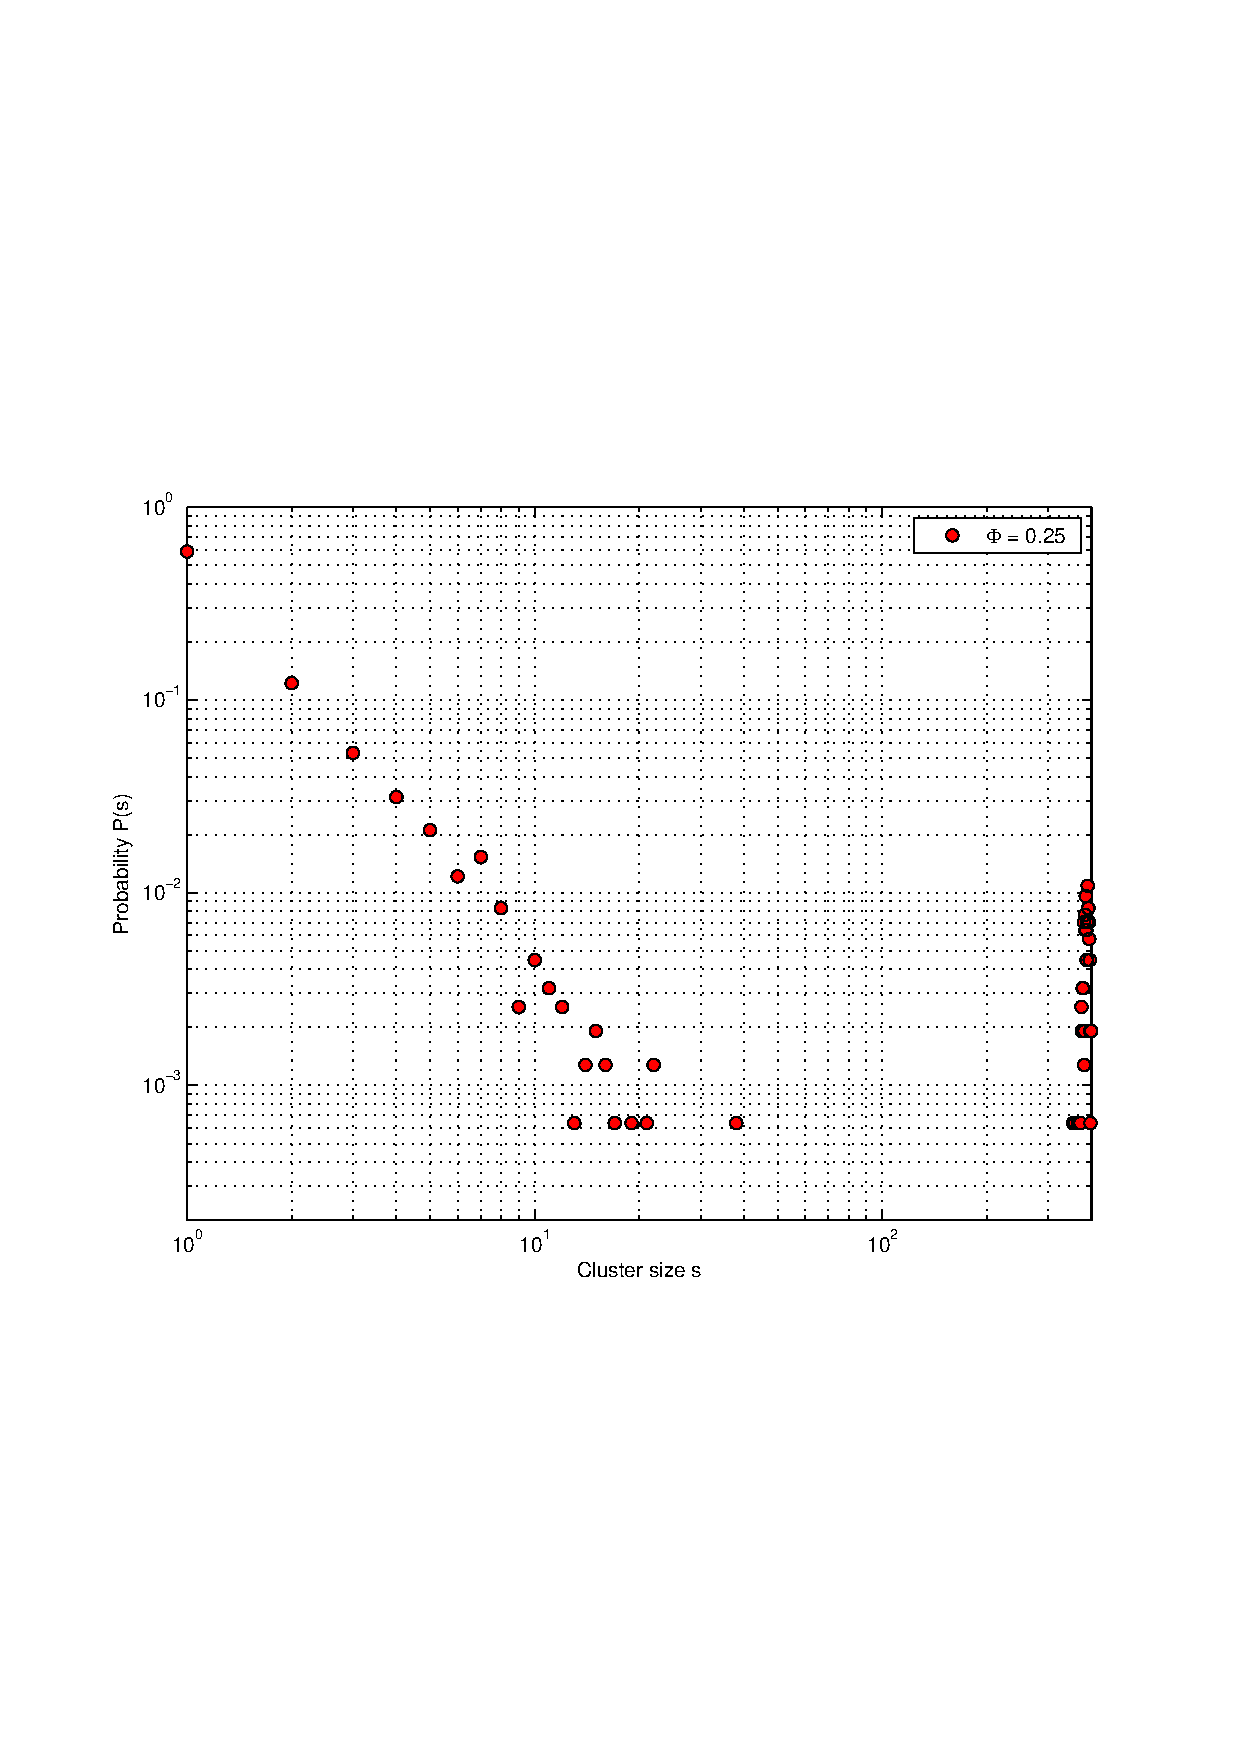
\includegraphics[scale=0.7]{Plots/S_Big.pdf}
  \caption{Cluster size distribution for $N=400$ at $\Phi<\Phi_c$.}
  \label{Fig:ClusterSizeBig}
\end{figure}

In the first plot of Fig. \ref{Fig:ClusterSizeBig}, one clearly sees power law distribution for small cluster size in the approximate range of $[1,20]$ as well as a peak near the maximal cluster size of $s=N$. We therefore refer to this scenario as the \textit{ordered phase}. It is quite remarkable that in the relatively wide range, approximately being $[40,300]$, no clusters are to be found. For low values of $s$ the data points agree well with a fitting line, whereas for higher values random fluctuation around the fit occur. This is simply due to the fact that the averaging works better for smaller cluster sizes because a certain value for a small cluster size is more likely to be obtained than for a bigger one. This fact is most pronounced in the region of the giant cluster. There the data points seem to be on top of each other, creating a sharp peak. In fact, each one of them sits on another value of $s$ that has been realized only a few times in all of the runs and thus is not averaged over many times.\\

\begin{figure}[h!]
  \centering
    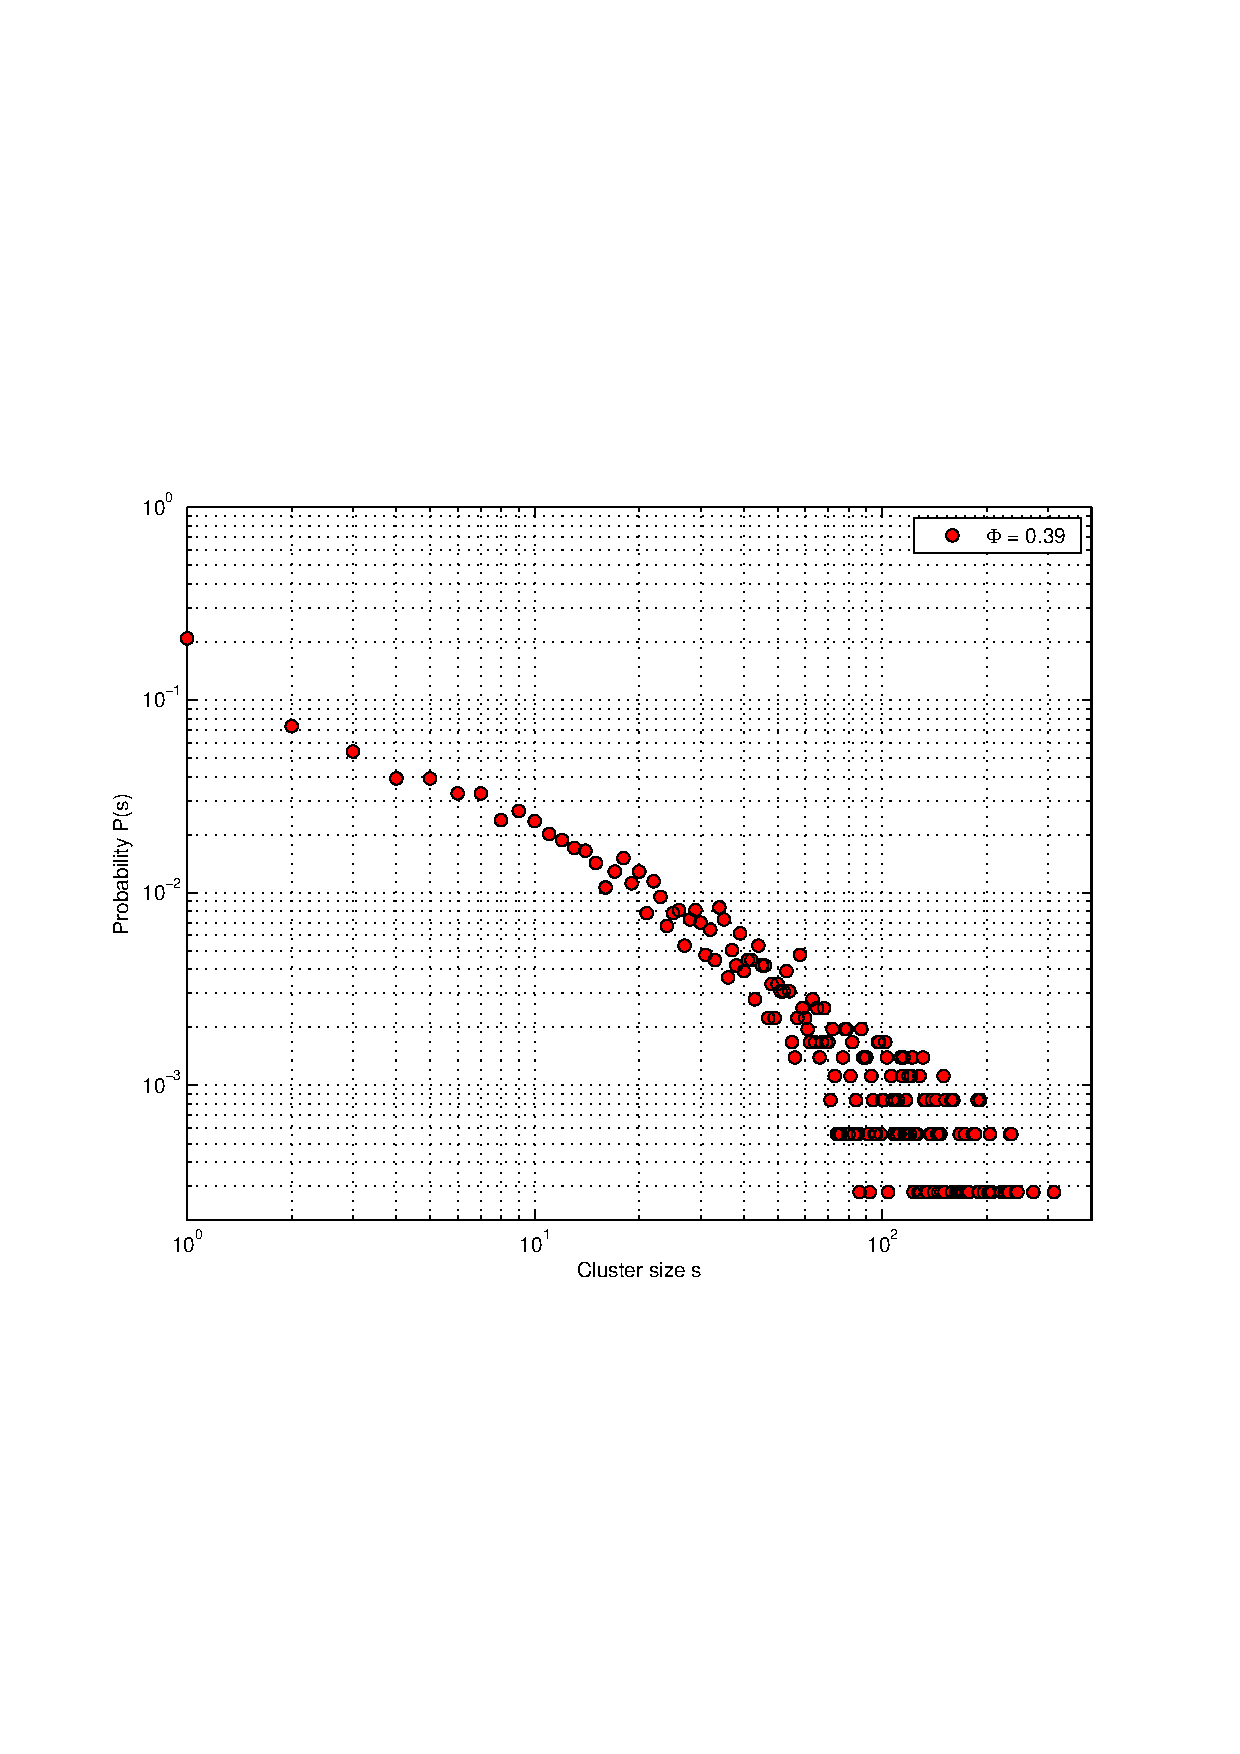
\includegraphics[scale=0.7]{Plots/S_Line.pdf}
  \caption{Cluster size distribution for $N=400$ at $\Phi \approx \Phi_c$.}
  \label{Fig:ClusterSizeCrit}
\end{figure}

Before turning our attention to the transition point, we discuss the third plot of Fig. \ref{Fig:ClusterSizePois}. Here the situation is very different as there is no giant cluster. In fact, the maximal cluster is smaller than $30$, which is less than 10\% of the giant cluster size for small $\Phi$ described above. Instead, the consensus state is marked by many small clusters. We therefore refer to this scenario as the \textit{unordered phase}. What strikes even more is the very smooth alignment of data points. The maximum of this distribution is approximately at $s=10$, which is exactly the value that was set for $\gamma$, i.e. the average number of nodes holding the same opinion. Upon analyzing a wide array of distributions for different system sizes (not shown here), it can be observed that the maximum of the unordered distribution is always at approximately $s=\gamma$. This is certainly no coincidence and can be explained as follows. For $\Phi$ close to unity only very few opinion changes are allowed. Consensus is achieved mostly entirely through reconnection. As $\gamma$ is set for the initial setup of the opinions, which will - due to the high value of $\Phi$ - barely change, the most likely cluster size will be exactly $\gamma$. This fact is shown for a specific value of $\Phi$ and $N$ but is independent of $N$ and $\Phi$ as long as the latter is above $\Phi_c$. Since the cluster size $s$ is given by the (integer) count of nodes in one cluster, the distribution can be considered as Poisson-like. This is also stated in the work of \cite{main paper}. 

In our case, however, the resemblence is certainly not perfect. Most notably, the tail at the lower end of the distribution performs an increase to another local maximum at $s=1$. Clusters of small size remain to be very likely to occur. The reason for this can be stated as follows: Small initial clusters in which members hold different opinions will reach local consensus very fast. The only chance for them to connect to other clusters to form bigger clusters, is that another node of the same opinion decides to reconnect to this small cluster. As for high $\gamma$ this is of course rather unlikely, smaller clusters remain "forever alone" in their local consensus state. This is most pronounced for lone nodes. They are in consensus by themselves and most unlikely to be connected to.\\


Now the question that remains to be answered, is \textit{how} and \textit{when} the transition between the two phases occurs. These can be answered when looking at the plot of \ref{Fig:ClusterSizeCrit}. A rather straight line that spans almost over the whole range of $s$ can be seen. The approximate value of $\Phi$ for which this occurs is $\Phi_c=0.39 \pm 0.05$, where the error has been estimated from visual judgement of the cluster size distributions. This is only a first guess and will be investigated in the following subsections. 

The curve combines aspects of both phases: there is a continuous distribution as well as a relatively big cluster, resulting in a power law distribution of clusters. This is an indicator for the continuous nature of the transition and is corroborated when considering the full range of $\Phi$ for the cluster size distribution. There it can be seen that for increasing $\Phi$ the giant cluster shrinks and smears out, thus closing the gap to the small clusters and forming the smooth straight line at the transition point. When further increasing $\Phi$ this straight line bends to form the Poisson-like distribution. \\

\begin{figure}[H]
  \centering
    \includegraphics[scale=0.7]{Plots/S_Pois.pdf}
  \caption{Cluster size distribution for $N=400$ at $\Phi>\Phi_c$.}
  \label{Fig:ClusterSizePois}
\end{figure}

In the following subsection \ref{Sec:Rescaling} the observation of a continuous phase transition will be further investigated and supported by further arguments. 
 

\subsection{Critical Point and Rescaling}
\label{Sec:Rescaling}

A more exact way of finding the critical point $\Phi_c$ is realized when altering the network size $N$. As stated in section \ref{Sec:Theory} different values for $N$ limit the range of interaction, i.e. the divergence of the coherence length, in the system. Therefore different critical exponents and hence different slopes around a point of intersection are observed. Smaller networks should be characterized by a less dramatic transition, i.e the slope at the critical value should be smaller than those of bigger networks. Qualitatively speaking, this is because in smaller networks it is more likely that a consensus state is achieved in the ordered phase without a very big giant cluster having formed. As a consequence the order parameter $S$ (which is introduced in this section) will on average be lower for smaller networks in the ordered phase. On the other hand, in the unordered phase the order parameter of smaller networks will on average be higher. This is because in smaller networks an equally often occurring reconnection is more likely to result in a bigger cluster. In short, closer to the thermodynamic limit of $N \rightarrow \infty$ the transition will be more ideal, i.e. more dramatic.

For these reasons and the intuition that the critical point should not depend on the system size (the boiling point of water is the same for 1ml and 10 ml), the point of intersection of the different curves for different $N$ can be interpreted as the wanted critical point $\Phi_c$. In Fig. \ref{Fig:SvsPHI} these curves are presented. In this figure each circle denotes a data point that was obtained from a cluster size distribution of the type presented in the previous subsection. From those distributions the size of the biggest cluster was divided by the network size, which yields the order parameter $S = s_{max}/N$. A sufficient amount of curves of different values of $N$ have been chosen such that the critical point is clearly visible. In general greater networks result in smoother curves. However, the computation exceeded reasonable limits, especially in the critical region (also see next subsection). Moreover, the difference of the curves becomes less and less visible. Hence, values for $N>400$ were not included. 

\begin{figure}[h!]
  \centering
    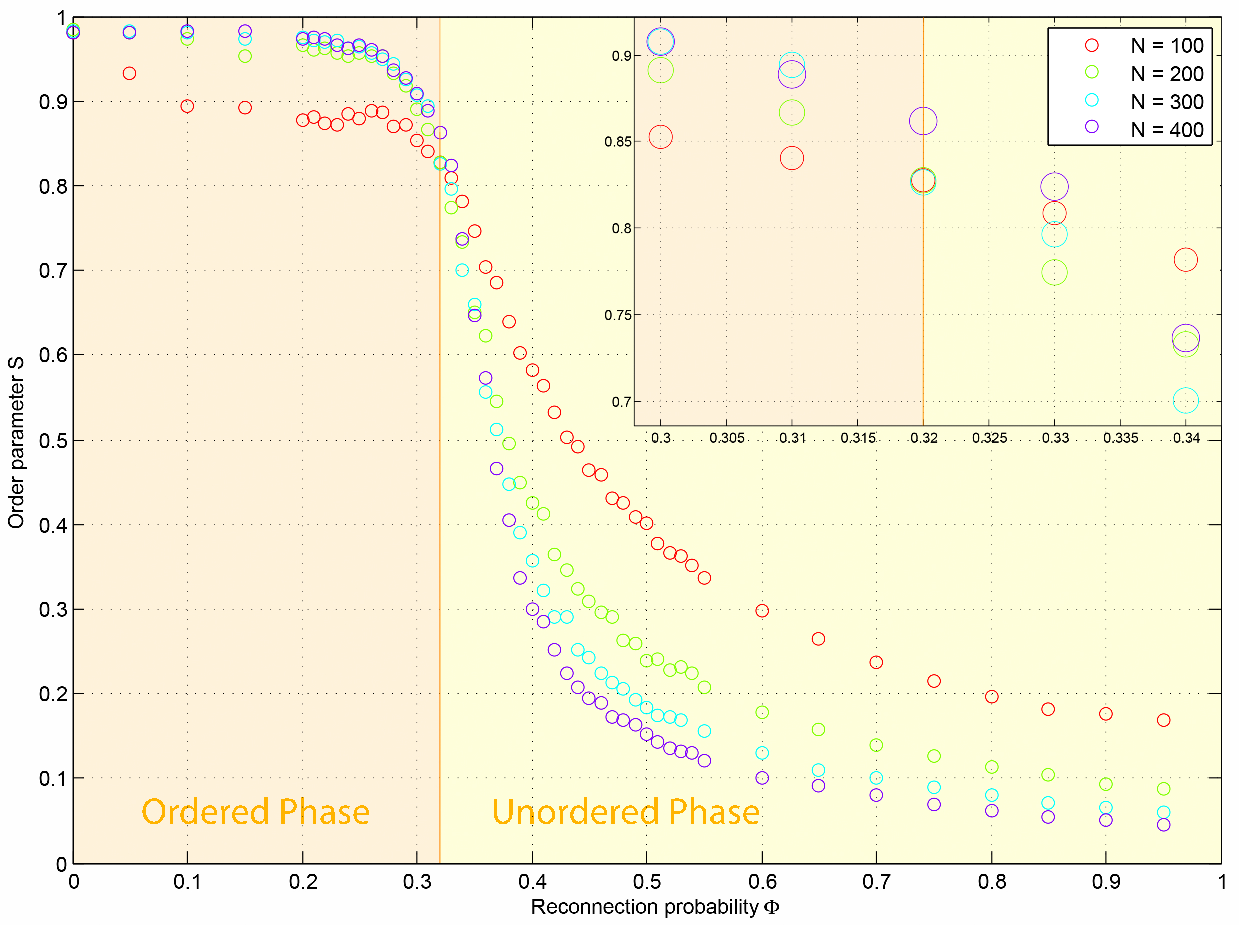
\includegraphics[scale=0.7]{Plots/SvsPHI_combined2.pdf}
  \caption{Order parameter versus reconnection probability for different network sizes.}
  \label{Fig:SvsPHI}
\end{figure}

The individual curves in the plot resemble those of a continuous phase transition. This is in agreement with the qualitative observation of the cluster size distribution in the previous subsection. A high order parameter marks the ordered phase, which is separated from the unordered phase (marked by a low order parameter) by the critical point. The critical point itself is found to be at $\Phi_c = 0.32 \pm 0.02$, where the error was estimated from the $\Phi$-steps taken and the relative overlap of data points near $\Phi=0.32$. This value does, however, not exactly agree with the value obtained in the previous subsection. In Fig. \ref{Fig:ClusterSizeCrit} the respective critical value is at $\Phi=0.39 \pm 0.05$. There is, in fact, an overlap at $\Phi=0.34$. But the following considerations will demonstrate that by applying the scaling laws introduced in section \ref{Sec:Theory} pretty much any value of $\Phi$ can be turned into a critical point. We will show this for the example of $\Phi=0.39$, also to reproduce the method used to quantitatively obtained the critical value in the work of \cite{main paper}.

\begin{figure}[h]
  \centering
    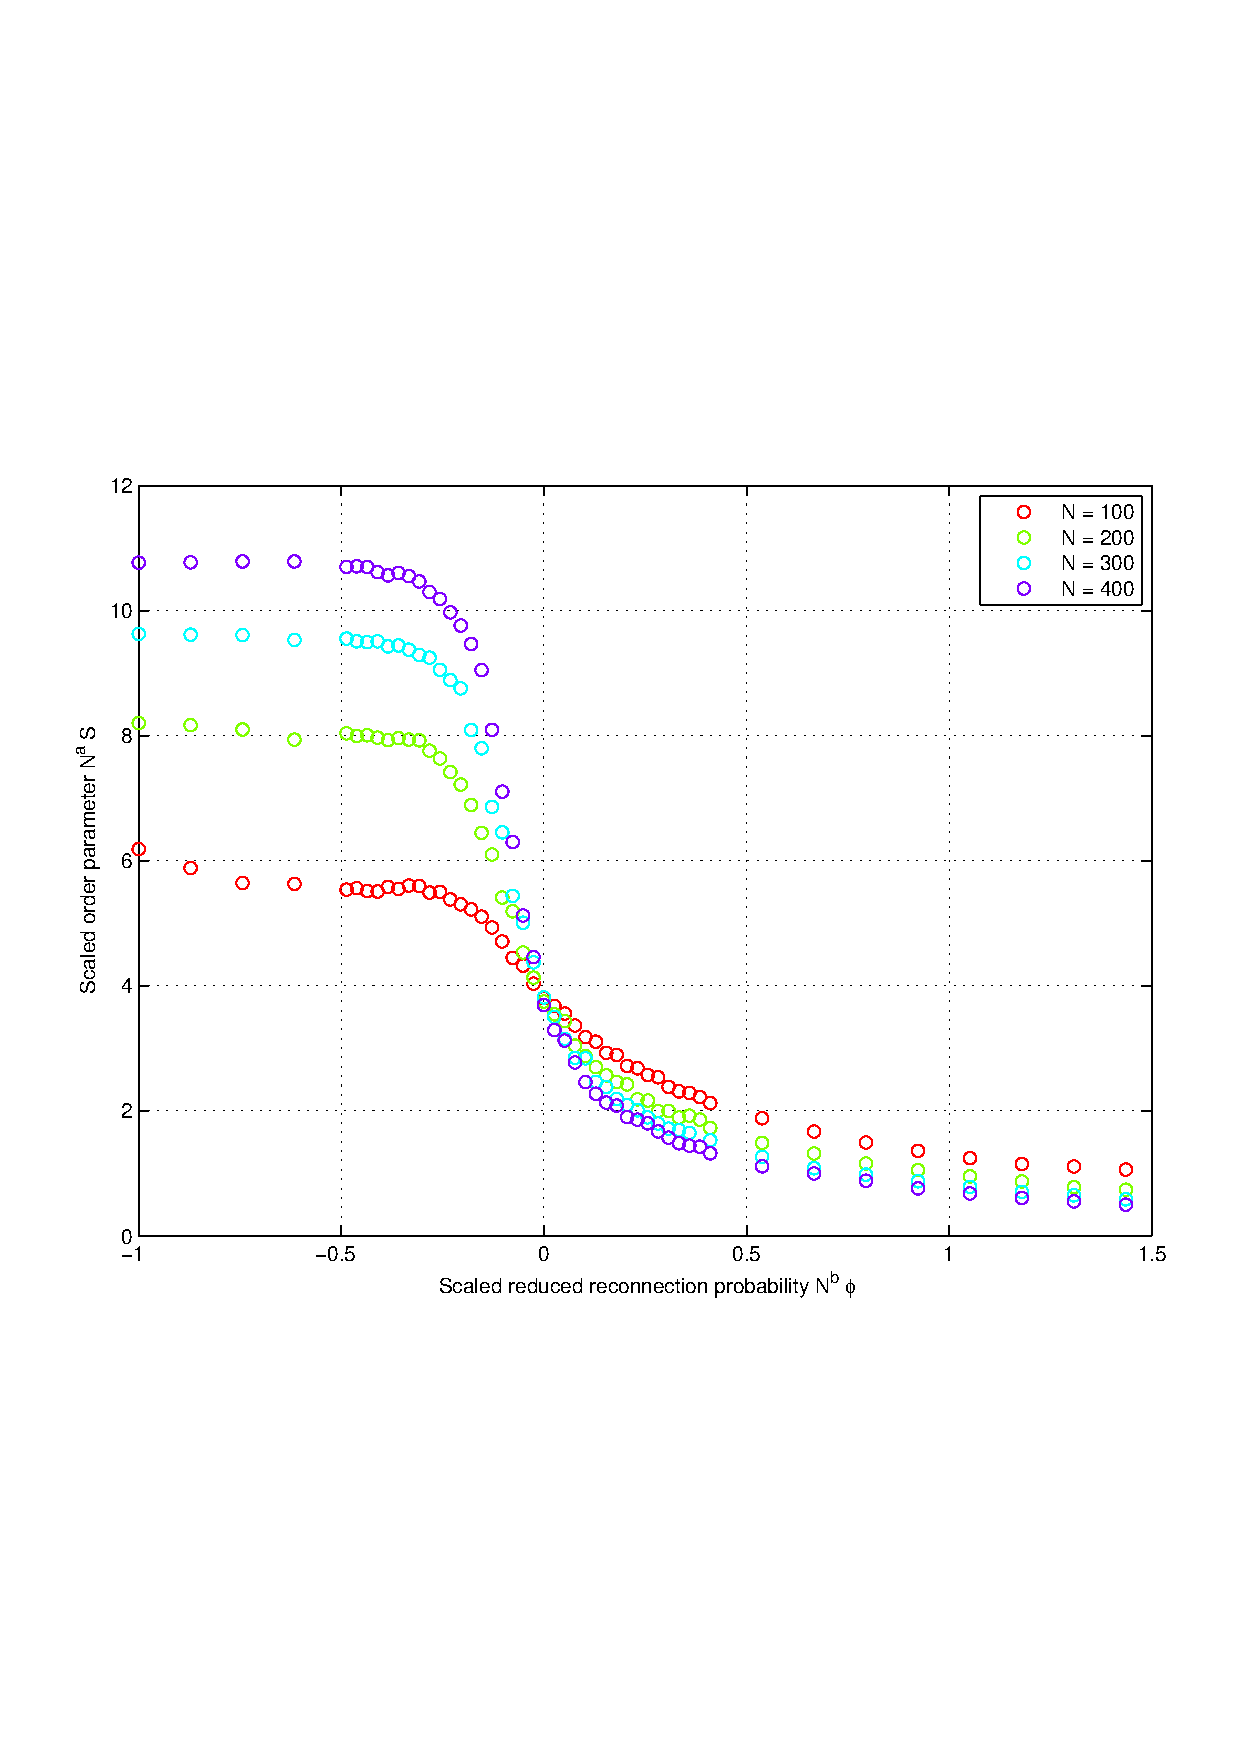
\includegraphics[scale=0.7]{Plots/SvsPHI2.pdf}
  \caption{Order parameter versus reconnection probability for different network sizes.}
  \label{Fig:phicrit2}
\end{figure}

In Fig. \ref{Fig:phicrit2} a rescaled order parameter, $N^a S$, was plotted against a rescaled reduced reconnection probability, $N^b \varphi$, according to \eqref{Eq:1paper}. In this form $a$ can be used to stretch or compress the curves in vertical direction depending on $N$, while $b$ can be used to do this in horizontal direction. Following the procedure outlined in the work of \cite{main paper}, first $a$ is tuned such that a neat point of intersection does occur at all and at $\varphi=0$. Without adapting $b$ (keeping it zero) yet, the resulting plot is shown for $a=0.4$ in Fig. \ref{Fig:phicrit2}. 

In the second step $b$ can be tuned such that the different $S(\varphi)$-curves collapse into one single curve near the transition point, indicating the independence of the system size $N$. This was already pointed out in section \ref{Sec:Theory} and is expressed in the fact that we get a single critical exponent $\alpha$ according to the \eqref{Eq:ab-powlaw}. This collapse of curves in the critical region was obtained for a value of $b=0.8$. The plot is presented in \ref{Fig:zoomed2}.

\begin{figure}[h!]
  \centering
    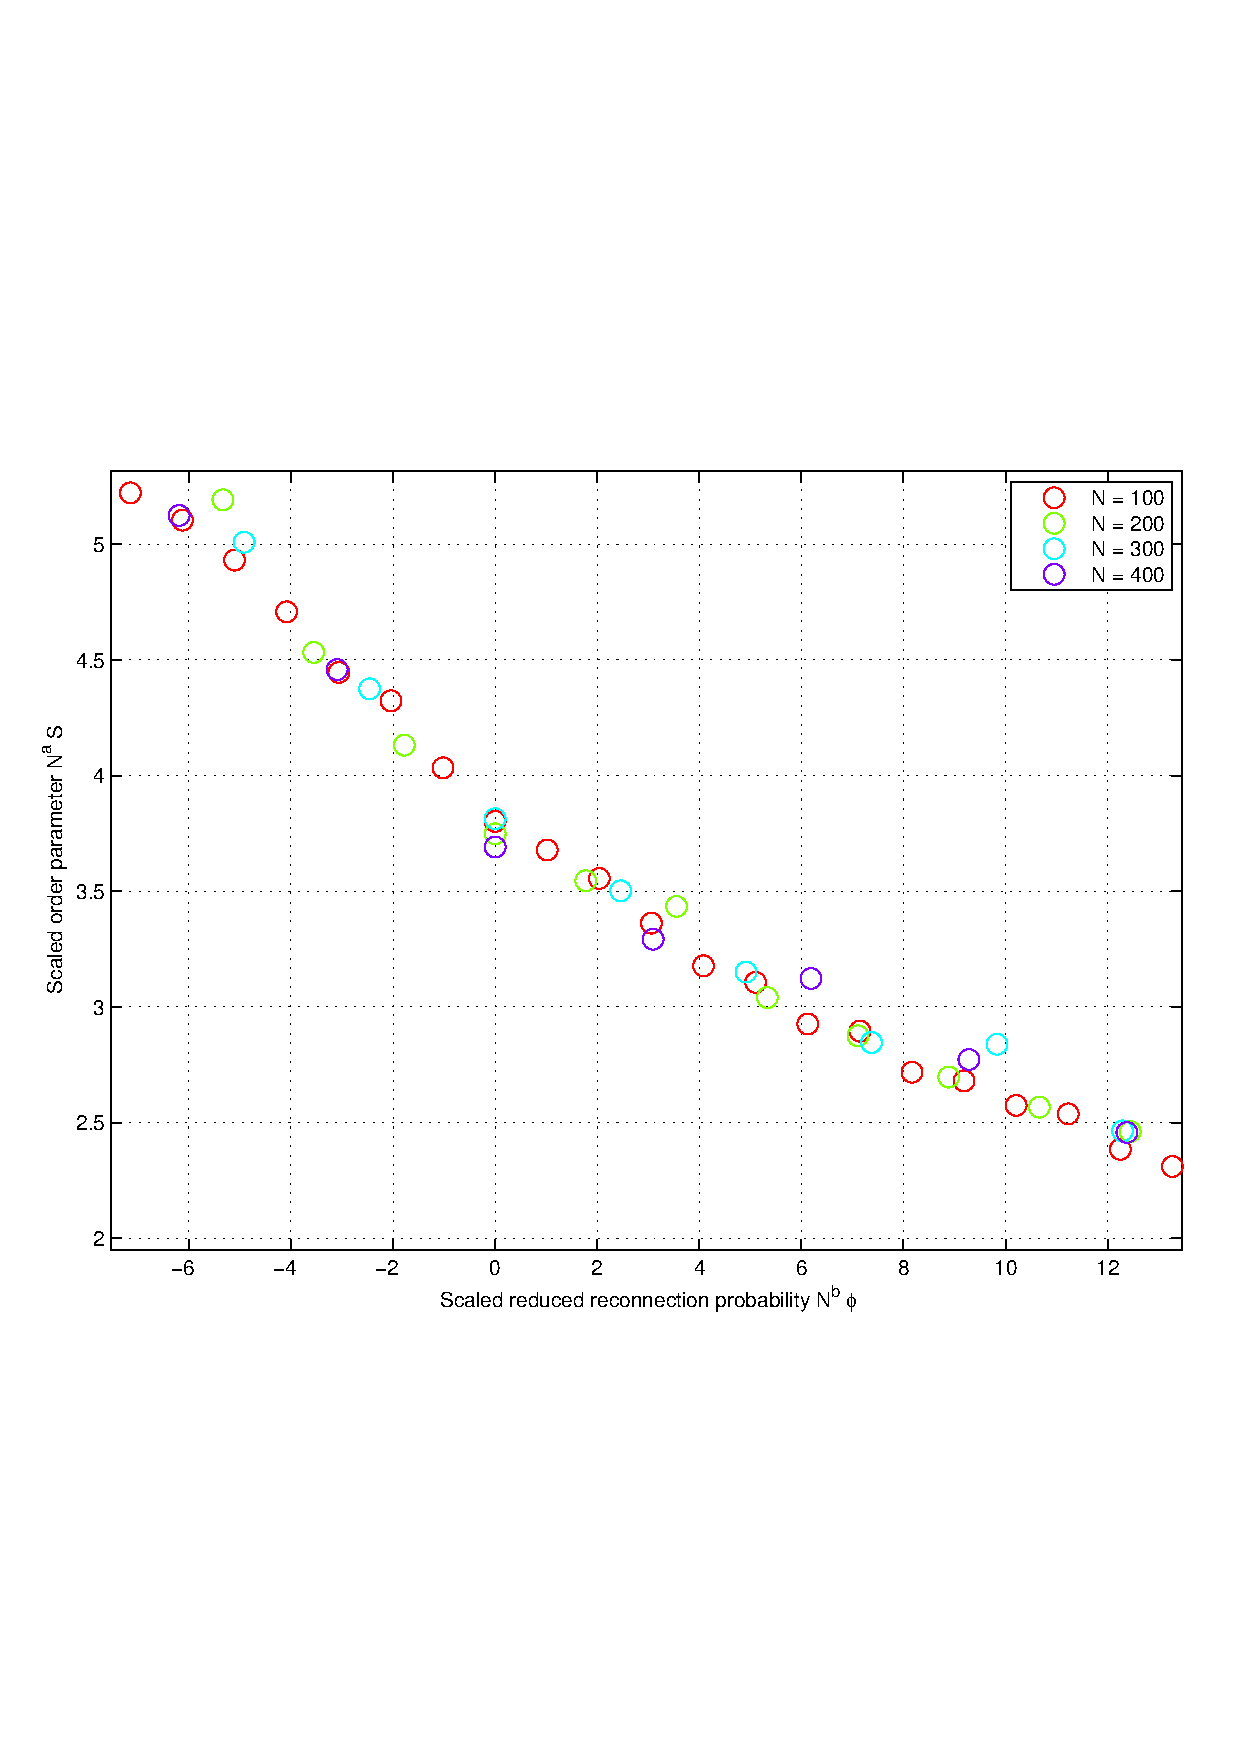
\includegraphics[scale=0.7]{Plots/SvsPHI2_zoom.pdf}
  \caption{Zoom into critical region of rescaled order parameter versus rescaled reduced reconnection probability. Here $a=0.4$ and $b=0.8$ such that the curves for different $N$ collapse into a single curve.}
  \label{Fig:zoomed2}
\end{figure}

Having determined $a$ and $b$, the critical exponent $\alpha$ could be calculated according to \eqref{Eq:ab-powlaw}. It turns out to be $\alpha=0.5$. This value is not presented with errors as this is a very crude if not arbitrary estimate. A comparison and assignment to universality classes of phase transitions would therefore not make any sense. Again, the calculation of $\alpha$ was mainly intended to reproduce the method of \cite{main paper} and to show that the calculation of a critical exponent is in theory possible. The main difference in our work is that we obtained a neat point of intersection without having to tune $a$ to a non-zero value. The only puzzling consequence is that this would correspond to a critical exponent of zero according to \eqref{Eq:powlaw}, which clearly cannot be the case.

The demonstrative example above was based on the indication of Fig. \ref{Fig:ClusterSizeCrit} that $\Phi_c = 0.39$. The fact that we do have a neat point of intersection of the $S(\varphi)$-curves and thus a relatively clear critical point of $\Phi_c=0.32$ is, however, stronger evidence. Additionally, the following subsection, which analyzes the convergence time of the system, provides even more evidence in favor of $\Phi_c=0.32$.

\subsection{Convergence Time}

The focus of our analysis was on the cluster size distribution and the arising phase transition. However, another interesting quantity is the relative average convergence time $\tau_{avg}$. This is the number of iterations relative to the number of nodes $N$ that the system takes (on average) to reach the consensus state. We initially recorded this quantity for each parameter combination and each run that we performed to optimize our simulation and parallelize the scripts most efficiently. However, upon plotting $\tau_{avg}$ in dependence of the reconnection probability $\Phi$, we noticed that it is also conceptually relevant. Fig. \ref{Fig:tau} shows a plot of $\tau_{avg}/N$ vs. $\Phi$ for different system sizes $N$.

\begin{figure}[h!]
  \centering
    \includegraphics[scale=0.8]{Plots/tau.pdf}
  \caption{Average time per node to reach consensus as a function of $\Phi$}
  \label{Fig:tau}
\end{figure}

It is clearly visible that the there is a value of $\Phi \approx 0.32$ at which the convergence time reaches a sharp peak which is approximately the same for all $N$. We can also observe that the peak convergence time and the time for low values of $\Phi$ is significantly larger the greater the system size, while for $\Phi \rightarrow 1$, we need roughly the same number of sweeps to reach consensus. More importantly, the peak seems to sharpen with increasing system size. \\

The sharpening of the peak and the shape of the curves as such bear a remarkable resemblance to divergent response functions or susceptibilities at the critical point as they appear in solid state physics. For physical systems, in fact, a divergent response function is part of the very definition of a phase transition. A divergence in such cases typically occurs in the (generally n-th order) derivative of some thermodynamic potential. For example, the magnetic susceptibility, which is proportional to the second derivative of the Helmholtz free energy with respect to magnetic field, diverges (i.e. becomes infinite in theory) at the critical temperature of a paramagnet-ferromagnet transition. This divergence, however, only occurs for infinitely large systems. For finite systems, the infinite peak broadens as the systems size is decreased. \\

Precisely this behavior can be seen (at least qualitatively) in our case, which reinforces our previous conclusion that the process of opinion and network formation in our model indeed obeys a phase transition. From this picture, we would obtain a critical probability $\Phi_c \approx 0.32 \pm 0.05$ which is not necessarily in agreement with the transition value determined in the previous section. However, as was already established, determining the critical point is very difficult with our given accuracy.  \\

Additionally, it is tempting to try to identify the convergence time of the network as some sort of response function or susceptibility, although it turned out to be difficult to find a straightforward physics analogy in this case. If we assume, as we did in section \ref{Sec:Theory}, that the reconnection probability $\Phi$ can be seen analogous to a temperature, it is very hard to point out a quantity in our system that corresponds to an external field. Also interpretations of $\tau_{avg}$ as a heat capacity or entropy are not very intuitive. Despite the difficulties to find an analogy to a response function, we remain confident that the peaks of the convergence time at the same critical value can hardly be a coincidence. Further investigations of this would certainly be interesting (see section \ref{Sec:summary}). \\

From a purely handwaving and intuitive point of view, however, it does make sense that the convergence time increases sharply at the (presumably) critical $\Phi_c$. After all, this is the point at which the two processes of opinion change and reconnection are in tough competition: What would otherwise be nearly a consensus state in the case of either small or large $\Phi$ is likely to be broken and pushed towards another phase by the respective other process, stretching the time until a consensus is reached. 


\subsection{Comparison with Empirical Data}

As what was proposed to be an optional task, we also set out to compare the results, i.e. the opinion size distribution, with actual data on opinions of a certain aspect, e.g. religious view. One could then think about by what factors our $\Phi$ is determined in reality and how to interpret it, if at all possible. Ideally, one could try to find data on the distribution of opinions, fit a function to it and based on the best match to the distribution of opinion cluster, determine the $\Phi$ that this real-world distribution situation corresponds to: An indicator for whether the opinion structure in question is formed rather by reconnection in the network or by adoption of opinions. \\

As already expected, getting "good" data that could be easily compared to theoretical predictions was not easy. Hence one possible simplification we thought of was instead of comparing entire distribution, it could also be an option to simply compare the size of the largest group of an opinion with our order parameter, which is a measure of exactly that. That way, only a single scalar value would have to be compared instead of a whole distribution function. \\

Due to the nature of the data, it also proved to be difficult to even generate cluster size histograms of the type in section \ref{Sec:cluster_distr} since in most real world cases just a handful of data points (opinions) even exist by the nature of the problem. For example, there is only a handful of mobile web browsers on the market. It is thus difficult to count the number of browsers of the same size since the count will always be one unless we significantly increase the binning interval. In such cases, we at least provided some qualitative observations and arguments. \\

As already argued in the introduction, our model is only applicable to generalized opinion structures that are mutually exclusive and "non-spectral", i.e. opinions exist independently without similarities. 

\subsubsection{Religious Views}

Since the analysis of the distribution of religious groups was the initial conceptual motivation of this project, we naturally tried to find sources to compare this type of data first. Getting reliable and finely-resolved statistics on religious adherence, however, is not an easy task. Also the definition of what the term "religion" entails varies from source to source. Especially when separating confessions into separate religions or aggregating them as one data point dramatically affects the distribution of sizes, which is exactly what we are trying to analyze and compare. \\

One already existing analysis is that of the total size distribution of religious communities globally, which happens to roughly follow a power law \cite{main paper} \cite{religion power law}. Fig. \ref{Fig:religion_power_law} (which is directly taken from \cite{religion power law}) shows this behavior. The paper cites the website "adherents.com" as the source of its data. \\


\begin{figure}[h!]
  \centering
    \includegraphics[scale=0.6]{Plots/religion_power_law.pdf}
  \caption{Size distribution of religious groups worldwide as found in \cite{religion power law}}
  \label{Fig:religion_power_law}
\end{figure}


In our model, we found a power law behavior of the cluster size distribution around the critical point! Comparing this to the empirical statistics would lead to the conclusion that religion is a critical phenomenon of opinion formation, of course under the assumption that our model is indeed applicable to reality. This would mean that the formation of religious views is not dominated by either of the two processes. \\

As already mentioned, finding further data for good quantitative analysis was rather difficult. However, without having to look at further data we can take the comparison to a qualitative argument: We know from experience that there are societies in which the distribution looks different and where one religion is completely dominating, for example in countries such as the USA or Saudi-Arabia. In such cases, the corresponding phase of our model would be the ordered one generated by a small reconnection probability $\Phi$, which means that individuals tend to adapt rather than reconnect. \\


Additionally, one needs to note that applying our model of opinion \emph{formation} to religion brings about some theoretical objections, e.g. that religion is an opinion that is rarely chosen freely (much less randomly) by an individual at some initial point. Thus the religious distribution within a region or country is unlikely to evolve significantly at all due to individual-level social processes. Thus we also thought of an alternative interpretation of "nodes" as families adhering to a particular religion, as already briefly mentioned in the introduction. In this interpretation, one could think of the process of opinion adoption as one where a family member changes his/her religion due to marrying a member of a family of different faith that he is connected with, thereby changing the religion of his/her entire family in the long term (on the time scale of a generation). On the other hand, a reconnection  would correspond to a family secluding itself from families of other religions. Keeping this in mind, one could think of the reconnection probability $\Phi$ as a kind of \emph{intolerance indicator} towards other religions: A low $\Phi$ would persist in a society in which intra-faith marriages are tolerated or even encouraged, while a high $\Phi$ would mean the opposite. \\


Looking at the results of our simulations, one could continue to say that a high intolerance indicator leads in the long term to a society in which one religion dominates strongly (ordered phase) while in a tolerant society, religions follow a much "softer" distribution (unordered or critical phase). While this may at first glance satisfy our intuition, one needs to be extremely careful with (potentially judgemental) conclusions such as "societies with a dominating religion are intolerant" since the validity of this interpretation is essentially speculation and very hard to prove. In fact, it is just as plausible to say that in the course of history borders of states were likely to be defined according to giant clusters of a religious view. Pakistan and India are prime examples for this.


\subsubsection{Mobile Web Browser Market Share}

A second possible interpretation of the generalized notion of "opinion" that our model could be applied to, is consumer preference or brand loyalty. In this subsection, the example of mobile web browser usage is analyzed. Under the (of course idealized and by no means obvious) assumption that all internet browsers for mobile devices are in fact objectively of equal quality, we can interpret an individual's choice in favor of one particular browser as an opinion. Since the individuals in a network of mobile browser users can be assumed to be socially interacting, we could try to compare such a scenario to our proposed model.

In doing so, we once again faced the problem of obtaining proper data that would be displayable in a histogram of cluster sizes. In essence, there are too few browsers to generate a meaningful histogram. Instead, we used the market shares of each browser as a proxy for the number of people who prefer one particular brand of mobile phone used to surf the web and make some qualitative arguments based on that. \\


\begin{figure}[h!]
  \centering
    \includegraphics[scale=0.6]{Plots/mobile_web.pdf}
  \caption{Time Development of Worldwide Market Shares for Mobile Web Browsers}
  \label{Fig:mobile_web}
\end{figure}


Fig. \ref{Fig:mobile_web} shows the development of these market shares between 2007 and 2009, taken from a report by Quantcast \cite{quantcast}. One can see that the distribution changes quite drastically with the introduction of Apple's iPhone: From what looks initially like a power law or Poisson distribution, the market arrives in a state in which one brand is very dominant. Unfortunately we were unable to find the raw data that was the basis of this plot, so it is not possible to establish what mathematical dependence is really present. Simply in terms of the largest market share, however, we might establish a connection to our order parameter: By the end of 2009, the largest competitor had a significant portion of the market share (ordered phase, small $\Phi$) while in mid-2007, it was much more evenly distributed (unordered phase, large $\Phi$). If this analogy can be made, we could interpret $\Phi$ as a kind of "brand disloyalty indicator" or even a quantity characterizing social influence: In the state of the market in 2009 (low $\Phi$), our corresponding dynamics in the model would assert that individuals are much more likely to adopt their friends' opinion (choice of phone brand), leading to a dominant cluster. Once again, though, this backward conclusion can only be stated as an assumption with the data available to us.\\

As a side note, it should be said that comparing different states of the market with different phases in our model can be problematic as such since our model only deals with \emph{equilibrium consensus states}, but this real world example is of course a continuously evolving and thus non-equilibrium system! By applying our model to it, we are essentially assuming some kind of equivalent to an adiabatic principle in thermodynamics: This would imply that at each time that we are measuring market shares, the underlying $\Phi$ has changed, causing the system to end up in a different convergent state. This assumption is of course a crude one that is hard to defend for real systems.



\section{Summary and Outlook}
\label{Sec:summary}

%different k values, gamma 
%spectral opinions: tune time evolutoin based on similarity of opinion (more likely to connect to a similiar opinion): start out with normal distribution (i.e. make extreme opinions less likely)
%introduce ``external field": informed agents that have a fixed opinion
%or: certain opinions are more likely to be switched to 
%superposed networks: one netw of religion, one of country

%we did shit differently than papaer: self and multi-edges!
%also different: we dont let i and j interact if they already have the same opinion (technically not what the paper says)

%There is a lot to be done in terms of applying physics-analogies to social systems. This might just be an example.

%Happy lone nodes: unrealistic. Nodes are social and should take the initiative to connect to others. In concrete k_avg should be allowed to increase.

%A proper interpretation of tau is still to be done!

%k and gamma dependencies --> Phase diagram



%Summary:

%First of all: PHASE TRANSITION AT ALL IST DER HAMMER!!!!
%critical exponent, what does it mean?
%We do get non-trivial opinion distribution (i.e. giant clusters)!

%Get back to the question and all that….

%Ideally: Find empirical distribution: Infer some phi --> we are there 
%Most countries have  giant cluster --> ppl dont like reconnecting?
%Religious families: phi as an intolerance indicator: high phi means i am unwilling to change my religion in order to sustain a friendship/marriage/whatever
%Brands: phi is a brand localty indicator: You are more likely to connect with people who have the same phone. Low phi: wert der marke ist bestimmt dadurch ob die neighboorhood auch diese brand hat

\subsection{Summary}

The initial motivation for this project was to investigate the interdependent evolution of opinions and networks by disentangling the combined process of one's social network shaping one's opinion and vice-versa. The central research question was whether our social surroundings determine which opinion we hold or whether our opinion determines whom we make part of our network and how these extremes influence the formation of networks and opinion structures.\\


In this work we were able to show that this general combined process can be modelled by setting a single parameter, the reconnection probability that gives the likelihood of an opinion holder to reconnect to a like-minded neighborhood versus adapting its opinion to its neighborhood. In other words this parameter determines the ratio with which each of two basic processes are realized. In different contexts the reconnection probability can be interpreted as a different real-life quantity. For example, an intolerance indicator influences the distribution of religious views in a country or region. In the context of consumer behavior a brand disloyalty indicator determines market shares of different brands of the same type of product. As the concept of a non-spectral opinions in social networks is very broad, many more examples are possible.\\


This work was in major parts an adaption of Holme's and Newman's work (\cite{main paper}). However, two essential parts were implemented differently. Firstly, while they were included in \cite{main paper} for reasons of simplicity, self- and multi-edges were forbidden in our model. Secondly, the explicitly does not alter local consensus states or "happy nodes". With this extended setup the most important results could be reproduced.\\


First of all and most remarkably, we found that a continuous phase transition occurs when gradually altering the reconnection probability. It is certainly non-trivial to have a giant cluster of equal opinion that at some point, around the critical value, suddenly is on equal standing with all the other opinions in the network. This trend was found to be increasingly pronounced for greater network sizes. The critical value for $k_{avg}=4$ and $\gamma=10$, which can be seen as measures of connection density and opinion diversity, respectively, was found to be $\Phi_c=0.32 \pm 0.05$. As a consequence of this critical region around this value, a network that is in a state of one dominating opinion, be it religion or brand, can in theory quite dramatically change to state in which this dominating opinion vanishes to a multitude of more or less equal opinions. What "dramatically" means in reality, depends on the context and can by no means be inferred from our model, which does not carry any information of (real) time or space.\\


Further, the analogies to statistical physics that could be drawn both qualitatively and quantitatively, are on the one hand hard to miss but should on the other hand be taken with caution. While it was possible to reproduce typical behaviour in thermodynamic systems, some predictions of the theory of critical phenomena could not be reproduced. The most notable analogy is the fact that for different network sizes, the phase transition curves of $S(\varphi)$ all intersect in the critical point. Furthermore, we could find a variable, the convergence time for reaching consensus, that diverges at this very critical point. Yet it is difficult to establish an analogy to divergent response functions in physics like the magnetic susceptibility. \\


Critical behavior in various systems is characterized and categorized by critical exponents which were attempted to be determined for the system in this work. It turned out that by strictly following the method suggested in \cite{main paper}, a wide range of values of $\Phi$ can be tuned to become the critical value. The tuning parameters $a$ and $b$ can be used to calculate a critical exponent, which in our exemplary calculation turned out to be $\alpha = 0.5$. In our case any of this tuning was not even necessary for obtaining a neat critical point, i.e. the trivial case of $a=b=0$ is just as well justifiable by this method. However, the puzzling consequence is that this would correspond to a critical value of zero, which is not in accordance to our qualitative findings and physical models.\\


\subsection{Outlook}

In future works there are vast possibilities to further investigate and extend the model in order to enable more analogies to statistical physics and its proven tools as well as to better account for reality. \\


The values of $k$ and $\gamma$ have been kept constant throughout this work. It would be of interest to investigate how a changing connectivity density and opinion diversity affects the critical reconnection probability and general behavior of the network. The work of \cite{main paper} suggests that $\Phi_c$ increases with $k$ but is constant with $\gamma$. But do those values need to be time-invariant at all? Networks could become more dense and diverse over time. \\


Speaking in physics terms, further state variables could enhance the applicability of physical models to this system. For example, a phase diagram could be established. It would be most expedient for this purpose to add to our "temperature" of the system, i.e. the reconnection probability, a "magnetic field". A most intuitive way to realize this is to introduce a finite number of nodes that hold a constant and equal opinion, penetrating the system like an externally applied field. In the work of \cite{informed agents} this was realized by including "informed agents" (nodes with constant opinion) in the network. However, this work was missing a temperature equivalent.\\


Another potentially far-reaching extension that can be added to the model is the spectrality of opinions. In this work only non-spectral opinions were considered. Yet there are many types of opinions that are much better described by \textit{spectral} opinions, i.e. opinion that are on a spectrum or continuum between extreme views. While religious views could on a larger time scale be argued to be of non-spectral type, it is certainly more intuitive to consider them as spectral opinions. It does make sense that certain religions are more similar to certain others. In order to account for this in our model, connecting or adapting to nodes of \textit{similar} as opposed to equal opinion has to be allowed and made dependent on the degree of similarity of opinions. In this sense it is also reasonable to initially distribute opinions in a way that favors opinions of central over extreme parts of the spectrum.

\begin{thebibliography}{9}

\bibitem{review}
R. Albert, A.-L. Barabasi. \emph{Statistical mechanics of complex
networks}. Rev. Mod. Phys, 74:47–98, 2002.

\bibitem{informed agents}
S. Brugger, C. Schwirzer. \emph{Opinion formation by "employed agents"
in social networks}. Project Report: Modelling and Simulating Social Systems with MATLAB, ETH Zurich, 2011.

\bibitem{voter model small world}
C. Castellano, D. Vilone, and A. Vespignani. \emph{Incomplete ordering
of the voter model on small-world networks}. Europhys.
Lett., 63:153–158, 2003.

\bibitem{erdos renyi}
P. Erd\H{o}s, A. R\'{e}nyi. \emph{On the evolution of random graphs}. Publications of the Mathematical Institute of the Hungarian Academy of Sciences 5: 17–61, 1960.

\bibitem{main paper}
P. Holme, M. E. J. Newman. \emph{Nonequilibrium phase transition in the coevolution of networks and opinions}. Physical Review E, vol. 74, Issue 5, id. 056108, 11/2006.

\bibitem{Nolting}
W. Nolting. \emph{Grundkurs Theoretische Physik 6: Statistische Physik}. Springer Berlin Heidelberg. 5. Aufl, 2004.

\bibitem{quantcast}
Quantcast, \emph{Quantcast Review of 2009 Mobile Web Trends}. "https://www.quantcast.com/inside-quantcast/2010/01/quantcast-review-of-2009-mobile-web-trends-mobile-web-share-up-110-in-north-america-and-148-globally" Accessed December 13, 2012.

\bibitem{voter model 2}
V. Sood, S. Redner. \emph{Voter model on heterogeneous graphs}. Phys. Rev. Lett., 94:178701, 2005.

\bibitem{religion power law}
D. H. Zanette,S. C. Manrubia. \emph{Vertical transmission of culture and the distribution of family names}. Physica A, 295:1–8, 2001.

\bibitem{ASSP}
A. Zheludev. \emph{Advanced solid state physics}. Lecture, ETH Zurich, Fall 2012.

\end{thebibliography}

\listoffigures

\newpage

\section{Appendix}

\subsection{Source Code}

\subsubsection{Main Script}
\lstinputlisting{code/main_script.m}


\subsubsection{Random Graph Generator}
\lstinputlisting{code/uniform_random_graph.m}


\subsubsection{Simulation}
\lstinputlisting{code/simulation.m}


\subsubsection{Cluster Size Distribution}
\lstinputlisting{code/clustersize_distr.m}


\subsubsection{Order Parameter Plotter}
\lstinputlisting{code/op_plotter_general.m}


\subsubsection{Convergence Time Plotter}
\lstinputlisting{code/tau_plotter.m}




\end{document}  



 
